% !TeX spellcheck = pl_PL
%%%%%%%%%%%%%%%%%%%%%%%%%%%%%%%%%%%%%%%%%%%
%                                        %
% Szablon pracy dyplomowej inzynierskiej %
% zgodny  z aktualnymi  przepisami  SZJK %
%                                        %
%%%%%%%%%%%%%%%%%%%%%%%%%%%%%%%%%%%%%%%%%%
%                                        %
%  (c) Krzysztof Simiński, 2018-2023     %
%                                        %
%%%%%%%%%%%%%%%%%%%%%%%%%%%%%%%%%%%%%%%%%%
%                                        %
% Najnowsza wersja szablonów jest        %
% podstępna pod adresem                  %
% github.com/ksiminski/polsl-aei-theses  %
%                                        %
%%%%%%%%%%%%%%%%%%%%%%%%%%%%%%%%%%%%%%%%%%
%
%
% Projekt LaTeXowy zapewnia odpowiednie formatowanie pracy,
% zgodnie z wymaganiami Systemu zapewniania jakości kształcenia.
% Proszę nie zmieniać ustawień formatowania (np. fontu,
% marginesów, wytłuszczeń, kursywy itd. ).
%
% Projekt można kompilować na kilka sposobów.
%
% 1. kompilacja pdfLaTeX
%
% pdflatex main
% bibtex   main
% pdflatex main
% pdflatex main
%
%
% 2. kompilacja XeLaTeX
%
% Kompilatacja przy użyciu XeLaTeXa różni się tym, że na stronie
% tytułowej używany jest font Calibri. Wymaga to jego uprzedniego
% zainstalowania.
%
% xelatex main
% bibtex  main
% xelatex main
% xelatex main
%
%
%%%%%%%%%%%%%%%%%%%%%%%%%%%%%%%%%%%%%%%%%%%%%%%%%%%%%
% W przypadku pytań, uwag, proszę pisać na adres:   %
%      krzysztof.siminski(małpa)polsl.pl            %
%%%%%%%%%%%%%%%%%%%%%%%%%%%%%%%%%%%%%%%%%%%%%%%%%%%%%
%
% Chcemy ulepszać szablony LaTeXowe prac dyplomowych.
% Wypełniając ankietę spod poniższego adresu pomogą
% Państwo nam to zrobić. Ankieta jest całkowicie
% anonimowa. Dziękujemy!


% https://docs.google.com/forms/d/e/1FAIpQLScyllVxNKzKFHfILDfdbwC-jvT8YL0RSTFs-s27UGw9CKn-fQ/viewform?usp=sf_link
%
%%%%%%%%%%%%%%%%%%%%%%%%%%%%%%%%%%%%%%%%%%%%%%%%%%%%%%%%%%%%%%%%%%%%%%%%%

%%%%%%%%%%%%%%%%%%%%%%%%%%%%%%%%%%%%%%%%%%%%%%%
%                                             %
% PERSONALIZACJA PRACY – DANE PRACY           %
%                                             %
%%%%%%%%%%%%%%%%%%%%%%%%%%%%%%%%%%%%%%%%%%%%%%%

% Proszę wpisać swoje dane w poniższych definicjach.

% TODO
% dane autora
\newcommand{\FirstNameAuthor}{Piotr}
\newcommand{\SurnameAuthor}{Kupczyk}
\newcommand{\IdAuthor}{305198}   % numer albumu  (bez $\langle$ i $\rangle$)

% drugi autor:
%\newcommand{\FirstNameCoauthor}{Imię}   % Jeżeli jest drugi autor, to tutaj należy podać imię.
%\newcommand{\SurnameCoauthor}{Nazwisko} % Jeżeli jest drugi autor, to tutaj należy podać nazwisko.
%\newcommand{\IdCoauthor}{$\langle$wpisać właściwy$\rangle$}  % numer albumu drugiego autora (bez $\langle$ i $\rangle$)
% Gdy nie ma drugiego autora, należy zostawić poniższe definicje puste, jak poniżej. Gdy jest drugi autor, należy zakomentować te linie.
\newcommand{\FirstNameCoauthor}{} % Jeżeli praca ma tylko jednego autora, to dane drugiego autora zostają puste.
\newcommand{\SurnameCoauthor}{}   % Jeżeli praca ma tylko jednego autora, to dane drugiego autora zostają puste.
\newcommand{\IdCoauthor}{}  % Jeżeli praca ma tylko jednego autora, to dane drugiego autora zostają puste.
%%%%%%%%%%

\newcommand{\Supervisor}{dr hab. inż. Bożena Małysiak-Mrozek}     % dane promotora (bez $\langle$ i $\rangle$)
\newcommand{\Title}{System wspomagający inteligentne składanie zestawów komputerowych}           % tytuł pracy po polsku
\newcommand{\TitleAlt}{A system supporting intelligent assembly of computer sets}                     % thesis title in English
\newcommand{\Program}{Teleinformatyka S1}            % kierunek studiów  (bez $\langle$ i $\rangle$)
\newcommand{\Specialisation}{Brak}     % specjalność  (bez $\langle$ i $\rangle$)
\newcommand{\Departament}{Systemów Rozproszonych i Urządzeń Informatyki}        % katedra promotora  (bez $\langle$ i $\rangle$)

% Jeżeli został wyznaczony promotor pomocniczy lub opiekun, proszę go/ją wpisać ...
\newcommand{\Consultant}{} % dane promotora pomocniczego, opiekuna (bez $\langle$ i $\rangle$)
% ... w przeciwnym razie proszę zostawić puste miejsce jak poniżej:
%\newcommand{\Consultant}{} % brak promotowa pomocniczego / opiekuna

% koniec fragmentu do modyfikacji
%%%%%%%%%%%%%%%%%%%%%%%%%%%%%%%%%%%%%%%%%%


%%%%%%%%%%%%%%%%%%%%%%%%%%%%%%%%%%%%%%%%%%%%%%%
%                                             %
% KONIEC PERSONALIZACJI PRACY                 %
%                                             %
%%%%%%%%%%%%%%%%%%%%%%%%%%%%%%%%%%%%%%%%%%%%%%%

%%%%%%%%%%%%%%%%%%%%%%%%%%%%%%%%%%%%%%%%


%%%%%%%%%%%%%%%%%%%%%%%%%%%%%%%%%%%%%%%%%%%%%%%
%                                             %
% PROSZĘ NIE MODYFIKOWAĆ PONIŻSZYCH USTAWIEŃ! %
%                                             %
%%%%%%%%%%%%%%%%%%%%%%%%%%%%%%%%%%%%%%%%%%%%%%%



\documentclass[a4paper,twoside,12pt]{book}
\usepackage[utf8]{inputenc}                                      
\usepackage[T1]{fontenc}  
\usepackage{amsmath,amsfonts,amssymb,amsthm}
\usepackage[british,polish]{babel} 
\usepackage{indentfirst}
\usepackage{xurl}
\usepackage{xstring}
\usepackage{ifthen}
\usepackage{float}



\usepackage{ifxetex}

\ifxetex
	\usepackage{fontspec}
	\defaultfontfeatures{Mapping=tex—text} % to support TeX conventions like ``——-''
	\usepackage{xunicode} % Unicode support for LaTeX character names (accents, European chars, etc)
	\usepackage{xltxtra} % Extra customizations for XeLaTeX
\else
	\usepackage{lmodern}
\fi



\usepackage[margin=2.5cm]{geometry}
\usepackage{graphicx} 
\usepackage{hyperref}
\usepackage{booktabs}
\usepackage{tikz}
\usepackage{pgfplots}
\usepackage{mathtools}
\usepackage{geometry}
\usepackage{subcaption}   % subfigures
\usepackage[page]{appendix} % toc,
\renewcommand{\appendixtocname}{Dodatki}
\renewcommand{\appendixpagename}{Dodatki}
\renewcommand{\appendixname}{Dodatek}


\usepackage{csquotes}
\usepackage[natbib=true,backend=bibtex,maxbibnames=99]{biblatex}  % kompilacja bibliografii BibTeXem
%\usepackage[natbib=true,backend=biber,maxbibnames=99]{biblatex}  % kompilacja bibliografii Biberem
\bibliography{biblio}

\usepackage{ifmtarg}   % empty commands  

\usepackage{setspace}
\onehalfspacing


\frenchspacing

%%%%%%%%%%%%%%%%%%%%%%%%%%%%%%%%%%
% środowiska dla definicji, twierdzenia, przykładu
\usepackage{amsthm}

\newtheorem{Definition}{Definicja}
\newtheorem{Example}{Przykład}
\newtheorem{Theorem}{Twierdzenie}
%%%%%%%%%%%%%%%%%%%%%%%%%%%%%%%%%%

%%%% TODO LIST GENERATOR %%%%%%%%%

\usepackage{color}
\definecolor{brickred}      {cmyk}{0   , 0.89, 0.94, 0.28}

\makeatletter \newcommand \kslistofremarks{\section*{Uwagi} \@starttoc{rks}}
  \newcommand\l@uwagas[2]
    {\par\noindent \textbf{#2:} %\parbox{10cm}
{#1}\par} \makeatother


\newcommand{\ksremark}[1]{%
{%\marginpar{\textdbend}
{\color{brickred}{[#1]}}}%
\addcontentsline{rks}{uwagas}{\protect{#1}}%
}

\newcommand{\comma}{\ksremark{przecinek}}
\newcommand{\nocomma}{\ksremark{bez przecinka}}
\newcommand{\styl}{\ksremark{styl}}
\newcommand{\ortografia}{\ksremark{ortografia}}
\newcommand{\fleksja}{\ksremark{fleksja}}
\newcommand{\pauza}{\ksremark{pauza `--', nie dywiz `-'}}
\newcommand{\kolokwializm}{\ksremark{kolokwializm}}
\newcommand{\cudzyslowy}{\ksremark{,,polskie cudzysłowy''}}

%%%%%%%%%%%%%% END OF TODO LIST GENERATOR %%%%%%%%%%%

\newcommand{\printCoauthor}{%		
    \StrLen{\FirstNameCoauthor}[\FNCoALen]
    \ifthenelse{\FNCoALen > 0}%
    {%
		{\large\bfseries\Coauthor\par}
	
		{\normalsize\bfseries \LeftId: \IdCoauthor\par}
    }%
    {}
} 

%%%%%%%%%%%%%%%%%%%%%
\newcommand{\autor}{%		
    \StrLen{\FirstNameCoauthor}[\FNCoALenXX]
    \ifthenelse{\FNCoALenXX > 0}%
    {\FirstNameAuthor\ \SurnameAuthor, \FirstNameCoauthor\ \SurnameCoauthor}%
	{\FirstNameAuthor\ \SurnameAuthor}%
}
%%%%%%%%%%%%%%%%%%%%%

\StrLen{\FirstNameCoauthor}[\FNCoALen]
\ifthenelse{\FNCoALen > 0}%
{%
\author{\FirstNameAuthor\ \SurnameAuthor, \FirstNameCoauthor\ \SurnameCoauthor}
}%
{%
\author{\FirstNameAuthor\ \SurnameAuthor}
}%

%%%%%%%%%%%% ZYWA PAGINA %%%%%%%%%%%%%%%
% brak kapitalizacji zywej paginy
\usepackage{fancyhdr}
\pagestyle{fancy}
\fancyhf{}
\fancyhead[LO]{\nouppercase{\it\rightmark}}
\fancyhead[RE]{\nouppercase{\it\leftmark}}
\fancyhead[LE,RO]{\it\thepage}


\fancypagestyle{tylkoNumeryStron}{%
   \fancyhf{} 
   \fancyhead[LE,RO]{\it\thepage}
}

\fancypagestyle{bezNumeracji}{%
   \fancyhf{} 
   \fancyhead[LE,RO]{}
}


\fancypagestyle{NumeryStronNazwyRozdzialow}{%
   \fancyhf{} 
   \fancyhead[LE]{\nouppercase{\autor}}
   \fancyhead[RO]{\nouppercase{\leftmark}} 
   \fancyfoot[CE, CO]{\thepage}
}


%%%%%%%%%%%%% OBCE WTRETY  
\newcommand{\obcy}[1]{\emph{#1}}
\newcommand{\english}[1]{{\selectlanguage{british}\obcy{#1}}}
%%%%%%%%%%%%%%%%%%%%%%%%%%%%%

% polskie oznaczenia funkcji matematycznych
\renewcommand{\tan}{\operatorname {tg}}
\renewcommand{\log}{\operatorname {lg}}

% jeszcze jakies drobiazgi

\newcounter{stronyPozaNumeracja}

%%%%%%%%%%%%%%%%%%%%%%%%%%% 
\newcommand{\printOpiekun}[1]{%		

    \StrLen{\Consultant}[\mystringlen]
    \ifthenelse{\mystringlen > 0}%
    {%
       {\large{\bfseries OPIEKUN, PROMOTOR POMOCNICZY}\par}
       
       {\large{\bfseries \Consultant}\par}
    }%
    {}
} 
%
%%%%%%%%%%%%%%%%%%%%%%%%%%%%%%%%%%%%%%%%%%%%%%
 
% Proszę nie modyfikować poniższych definicji!
\newcommand{\Author}{\FirstNameAuthor\ \MakeUppercase{\SurnameAuthor}} 
\newcommand{\Coauthor}{\FirstNameCoauthor\ \MakeUppercase{\SurnameCoauthor}}
\newcommand{\Type}{PROJEKT INŻYNIERSKI}
\newcommand{\Faculty}{Wydział Automatyki, Elektroniki i Informatyki} 
\newcommand{\Polsl}{Politechnika Śląska}
\newcommand{\Logo}{politechnika_sl_logo_bw_pion_pl.pdf}
\newcommand{\LeftId}{Nr albumu}
\newcommand{\LeftProgram}{Kierunek}
\newcommand{\LeftSpecialisation}{Specjalność}
\newcommand{\LeftSUPERVISOR}{PROWADZĄCY PRACĘ}
\newcommand{\LeftDEPARTMENT}{KATEDRA}
%%%%%%%%%%%%%%%%%%%%%%%%%%%%%%%%%%%%%%%%%%%%%%

%%%%%%%%%%%%%%%%%%%%%%%%%%%%%%%%%%%%%%%%%%%%%%%
%                                             %
% KONIEC USTAWIEŃ                             %
%                                             %
%%%%%%%%%%%%%%%%%%%%%%%%%%%%%%%%%%%%%%%%%%%%%%%




%%%%%%%%%%%%%%%%%%%%%%%%%%%%%%%%%%%%%%%%%%%%%%%
%                                             %
% MOJE PAKIETY, USTAWIENIA ITD                %
%                                             %
%%%%%%%%%%%%%%%%%%%%%%%%%%%%%%%%%%%%%%%%%%%%%%%

% Tutaj proszę umieszczać swoje pakiety, makra, ustawienia itd.


 
%%%%%%%%%%%%%%%%%%%%%%%%%%%%%%%%%%%%%%%%%%%%%%%%%%%%%%%%%%%%%%%%%%%%%
% listingi i fragmentu kodu źródłowego 
% pakiet: listings lub minted
% % % % % % % % % % % % % % % % % % % % % % % % % % % % % % % % % % % 

% biblioteka listings
\usepackage{listings}
\lstset{%
morekeywords={system, wspomagający, inteligentne, składanie , zestawów , komputerowych, html, css, sql, model, logiczny, relacyjny, aplikacja, www, strona}% słowa kluczowe rozpoznawane przez pakiet listings
language=C++,% C, Matlab, Python, SQL, TeX, XML, bash, ... – vide https://www.ctan.org/pkg/listings
commentstyle=\textit,%
identifierstyle=\textsf,%
keywordstyle=\sffamily\bfseries, %\texttt, %
%captionpos=b,%
tabsize=3,%
frame=lines,%
numbers=left,%
numberstyle=\tiny,%
numbersep=5pt,%
breaklines=true,%
escapeinside={@*}{*@},%
}

% % % % % % % % % % % % % % % % % % % % % % % % % % % % % % % % % % % 
% pakiet minted
%\usepackage{minted}

% pakiet wymaga specjalnego kompilowania:
% pdflatex -shell-escape main.tex
% xelatex  -shell-escape main.tex

%\usepackage[chapter]{minted} % [section]
%%\usemintedstyle{bw}   % czarno-białe kody 
%
%\setminted % https://ctan.org/pkg/minted
%{
%%fontsize=\normalsize,%\footnotesize,
%%captionpos=b,%
%tabsize=3,%
%frame=lines,%
%framesep=2mm,
%numbers=left,%
%numbersep=5pt,%
%breaklines=true,%
%escapeinside=@@,%
%}

%%%%%%%%%%%%%%%%%%%%%%%%%%%%%%%%%%%%%%%%%%%%%%%%%%%%%%%%%%%%%%%%%%%%%



%%%%%%%%%%%%%%%%%%%%%%%%%%%%%%%%%%%%%%%%%%%%%%%
%                                             %
% KONIEC MOICH USTAWIEŃ                       %
%                                             %
%%%%%%%%%%%%%%%%%%%%%%%%%%%%%%%%%%%%%%%%%%%%%%%



%%%%%%%%%%%%%%%%%%%%%%%%%%%%%%%%%%%%%%%%


\begin{document}
%\kslistofremarks

\frontmatter

%%%%%%%%%%%%%%%%%%%%%%%%%%%%%%%%%%%%%%%%%%%%%%%
%                                             %
% PROSZĘ NIE MODYFIKOWAĆ STRONY TYTUŁOWEJ!    %
%                                             %
%%%%%%%%%%%%%%%%%%%%%%%%%%%%%%%%%%%%%%%%%%%%%%%


%%%%%%%%%%%%%%%%%%  STRONA TYTUŁOWA %%%%%%%%%%%%%%%%%%%
\pagestyle{empty}
{
	\newgeometry{top=1.5cm,%
	             bottom=2.5cm,%
	             left=3cm,
	             right=2.5cm}
 
	\ifxetex 
	  \begingroup
	  \setsansfont{Calibri}
	   
	\fi 
	 \sffamily
	\begin{center}
	\includegraphics[width=50mm]{\Logo}
	 
	
	{\Large\bfseries\Type\par}
	
	\vfill  \vfill  
			 
	{\large\Title\par}
	
	\vfill  
		
	{\large\bfseries\Author\par}
	
	{\normalsize\bfseries \LeftId: \IdAuthor}

	\printCoauthor
	
	\vfill  		
 
	{\large{\bfseries \LeftProgram:} \Program\par} 
	
	{\large{\bfseries \LeftSpecialisation:} \Specialisation\par} 
	 		
	\vfill  \vfill 	\vfill 	\vfill 	\vfill 	\vfill 	\vfill  
	 
	{\large{\bfseries \LeftSUPERVISOR}\par}
	
	{\large{\bfseries \Supervisor}\par}
				
	{\large{\bfseries \LeftDEPARTMENT\ \Departament} \par}
		
	{\large{\bfseries \Faculty}\par}
		
	\vfill  \vfill  

    	
    \printOpiekun{\Consultant}
    
	\vfill  \vfill  
		
    {\large\bfseries  Gliwice \the\year}

   \end{center}	
       \ifxetex 
       	  \endgroup
       \fi
	\restoregeometry
}
  
%%%%%%%%%%%%%%%%%%%%%%%%%%%%%%%%%%%%%%%%%%%%%%%
%                                             %
% KONIEC STRONY TYTUŁOWEJ                     %
%                                             %
%%%%%%%%%%%%%%%%%%%%%%%%%%%%%%%%%%%%%%%%%%%%%%%  


\cleardoublepage

\rmfamily\normalfont
\pagestyle{empty}


%%% No to zaczynamy pisać pracę :-) %%%%

% TODO
\subsubsection*{Tytuł pracy} 
\Title

\subsubsection*{Streszczenie}  
(Streszczenie pracy – odpowiednie pole w systemie APD powinno zawierać kopię tego streszczenia.)

\subsubsection*{Słowa kluczowe} 
(2-5 slow (fraz) kluczowych, oddzielonych przecinkami)

\subsubsection*{Thesis title} 
\begin{otherlanguage}{british}
\TitleAlt
\end{otherlanguage}

\subsubsection*{Abstract} 
\begin{otherlanguage}{british}
(Thesis abstract – to be copied into an appropriate field during an electronic submission – in English.)
\end{otherlanguage}
\subsubsection*{Key words}  
\begin{otherlanguage}{british}
(2-5 keywords, separated by commas)
\end{otherlanguage}




%%%%%%%%%%%%%%%%%% SPIS TRESCI %%%%%%%%%%%%%%%%%%%%%%
% Add \thispagestyle{empty} to the toc file (main.toc), because \pagestyle{empty} doesn't work if the TOC has multiple pages
\addtocontents{toc}{\protect\thispagestyle{empty}}
\tableofcontents

%%%%%%%%%%%%%%%%%%%%%%%%%%%%%%%%%%%%%%%%%%%%%%%%%%%%%
\setcounter{stronyPozaNumeracja}{\value{page}}
\mainmatter
\pagestyle{empty}

\cleardoublepage

\pagestyle{NumeryStronNazwyRozdzialow}

%%%%%%%%%%%%%% wlasciwa tresc pracy %%%%%%%%%%%%%%%%%

% TODO
\chapter{Wstęp}
\label{ch:wstep}
\newpage
%%\begin{itemize}
%%\item wprowadzenie w problem/zagadnienie
%%\item osadzenie problemu w dziedzinie
%%\item cel pracy
%%\item zakres pracy
%%\item zwięzła charakterystyka rozdziałów
%%\item jednoznaczne określenie wkładu autora, w przypadku prac wieloosobowych – tabela z autorstwem poszczególnych elementów pracy
%%\end{itemize}

\section{Wprowadzenie w problem}
Sklepy komputerowe zazwyczaj posiadają swój własny sklep internetowy, oferujący możliwość zakupów części indywidualnie, jak i gotowych zestawów PC. Odpowiedni dobór komponentów jest najistotniejszą częscią procesu projetkowania własnego stanowiska, a pomimo tego najwięksi sprzedawcy nie oferują możliwości sprawdzania kompatybilności wybranych produktów. Dlatego projekt ma na celu stworzenie prostej i intuicyjnej strony internetowej, która zaoferuje przystępną formę weryfikacji poprawności wyboru komponentów z katalogu oraz finalnie dodanie kompatybilnego zestawu do koszyka użytkownika. 

\section{Osadzenie problemu w dziedzinie}
Projekt osadzony jest w dziedzinie inżynierii oprogramowania, projektowania baz danych oraz systemów e-commerce. Praca obejmuje zagadnienia relacyjności baz danych, budowy warstwy komunikacyjnej backendu, implementacji logiki aplikacji pod kątem biznesowym oraz wdrożenie interfejsu frontendowego.

\section{Cel pracy}

Celem pracy jest zaprojektowanie i zaimplementowanie aplikacji webowej, która będzie pełnić funkcję inteligentnego kreatora zestawów komputerowych. System będzie dawać użytkownikowi możliwosć wybrania dowolnych produktów z katalogu, sprawdzenie czy aktualne zamówienie jest wzajemnie kompatybilne, a gdy weryfikacja zakończy się pomyślnie, umożliwi realizację zamównienia. 
\newpage
Idące za tym cele to:
\begin{itemize} 
	\item stworzenie relacyjnej bazy danych, odpowiadającej potrzebom sklepu internetowego,
	\item zaprojektowanie i implementacja backendu, odpowiedzialnego za komunikację i logikę aplkacji, 
	\item wdrożenie przejrzystego frontendu, będącego interfejsem klienta,
	\item stworzenie grupy zasobów w środowisku chmurowym Azure (baza danych jako storage, aplikacja jako kontener).
\end{itemize}
\section{Zakres pracy}
Zakres pracy nad projektem obejmuje:
\begin{itemize}
	\item projekt relacyjnej bazy danych w Oracle SQL Developer.
	\item utworzenie testowego serwera PostgreSQL, wprowadzenie gotowych danych o produktach do bazy danych,
	\item stworzenie użytkowników oraz nadanie odpowiednich uprawnień każdemu z nich,
	\item implementację backendu w języku Python, implementacja API z wykorzystaniem frameworka FastAPI, umożliwiając integrację z bazą danych w celu zarządzania produktami i zamówieniami,
	\item projekt interfejsu użytkownika, stworzenie frontendu używając HTML, CSS oraz JavaScript,
	\item projekt kreatora zestawów komputerowych, zaimplementowanego z uwzględnieniem logik rozmytej, używając Reacta, Typescript, Node.js,
	\item migrację gotowej aplikacji z lokalnego serwera testowego PostgreSQL do produkcyjnej chmury Azure, utworzenie grupy zasobów.
	
\end{itemize}
\newpage
\section{Zwięzła charakterystyka rozdziałów}

\begin{itemize}
    \item \textbf{Rozdział 1} - zawiera wprowadzenie do tematyki pracy, przedstawia problem nieintuicyjnego doboru kompatybilnych podzespołów komputerowych, definiuje cel i zakres pracy oraz opisuje autorski wkład w projekt.

    \item \textbf{Rozdział 2} - obejmuje analizę tematu, w tym istotę kompatybilności sprzętowej, przegląd istniejących rozwiązań wykorzystywanych przez popularne sklepy komputerowe oraz porównanie ich funkcjonalności z zaprojektowanym systemem. Przybliża problematykę całej pracy.

    \item \textbf{Rozdział 3} - przedstawia wymagania funkcjonalne i niefunkcjonalne systemu, przypadki użycia, zastosowane narzędzia i technologie oraz metodykę pracy przyjętą podczas implementacji. Przedstawia kompletną listę dobranych technologii i rozwiązań.

    \item \textbf{Rozdział 4} - stanowi część projektową, zawierającą architekturę systemu, opisanie każdego filaru aplikacji webowej, model danych wraz z diagramem ERD, opis struktury bazy danych, szczegółową analizę encji oraz omówienie kluczowych modułów, takich jak moduł weryfikacji kompatybilności i logiki rozmytej.

    \item \textbf{Rozdział 5} - prezentuje proces weryfikacji i walidacji systemu, zawierając opis sposobu testowania, organizacji eksperymentów, przypadków testowych oraz analizę wykrytych błędów i wyników testów. Analizuje skuteczność działania oprogramowania, porównując otrzymywane wyniki z założeniami.

    \item \textbf{Rozdział 6} - zawiera podsumowanie uzyskanych rezultatów, ocenę stopnia realizacji celów pracy oraz wskazuje możliwe kierunki dalszego rozwoju systemu. Podsumowuje i ocenia skuteczność podjętych działań, analizuje koszty poniesione poczas realizacji, szczegołowo ocenia dobór technologii.
\end{itemize}


\newpage
\section{Wkład autora}
Autor samodzielnie opracował wszystkie elementy projektu, zaczynając od zaplanowania funkcjonalności oraz wyborze technologii. Następnym krokiem było zaprojektowanie relacyjnej bazy danych w Oracle SQL Developer, gdzie utworzył on testowy serwer PostgreSQL wraz z użytkownikami oraz nadał odpowiednie uprawnienia każdemu z nich. Przy użyciu frameworku FastAPI przygotowany został backend w języku Python, odpowiadający za komunikację z bazą danych oraz za logikę całej aplikacji, umożliwiając weryfikację kompatybilności zestawów komputerowych. Autor utworzył interaktywny frontend, który umożliwia graficzne korzystanie z aplikacji, zapewniając łatwość użytkowania zarówno dla doświadczonych, jak i początkujących inżynierów sprzętu, poprzez stosowanie logiki rozmytej. Korzystając z akademickiej subskrypcji Microsoft Azure autor używając otrzymanych kredytów samodzielnie realizuje hosting, administrację, testowanie CI/CD, konteneryzację oraz wirtualizację aplikacji webowej, czyniąc ją w pełni używalną w publicznej sieci internet. Dokumentacja przygotowana do projektu, dokument inzynierski oraz wszystkie opisy dostępne w projekcie zostały samodzielnie, szczegółowo opracowane w ramach projektu inzynierskiego "System wspomagający inteligentne składanie zestawów komputerowych".

\chapter{Analiza problemu oraz przegląd dostępnych rozwiązań}
\newpage
%%\begin{itemize}
%%\item sformułowanie problemu
%%\item osadzenie tematu w kontekście aktualnego stanu wiedzy (\english{state of the art}) o poruszanym problemie
%%\item  studia literaturowe \cite{bib:artykul,bib:ksiazka,bib:konferencja,bib:internet} -  opis znanych rozwiązań (także opisanych naukowo, jeżeli problem jest poruszany w publikacjach naukowych), algorytmów, 
%%%\end{itemize}


%%Wzory  
%%\begin{align}
%%y = \frac{\partial x}{\partial t}
%%\end{align}
%%jak i pojedyncze symbole $x$ i $y$  składa się w trybie matematycznym.

\section{Sformułowanie problemu}
\subsection{Istota kompatybilności}
Na rynku znajduje się szeroka gama komponentów komputerowych, która nieustannie poszerza się o nowe produkty. Różnice pomiędzy poszczególnymi modelami dotyczą chociażby wymiarów fizycznych, dostępnych złączy, technologi socketów, minimalnej mocy zasilacza, aż do wymogów software'owych. Odpowiedni dobór części jest pierwszym krokiem do realizacji poprawnie funkcjonującego stanowiska komputerowego, gdyż dowolna pomyłka może prowadzić do braku możliwości fizycznego montażu lub niewłaściwej i nieciągłej pracy urządzenia. Nawet minimalne niezgodności mogą być przyczyną poważnej awarii, która może przyczynić się do strat finansowych, spowodowanych utratą danych, przerwaniem trwałości usług lub całkowitym uszkodzeniem sprzętu.

\subsection{Niska dostępność narzędzi do weryfikacji kompatybilności}

Aktualnie na polskim rynku sklepów komputerowych brakuje narzędzi umożliwiających użytkownikowi samodzielną i automatyczną weryfikację kompatybilności wybranych podzespołów. Większość sprzedawców oferuje wyłącznie gotowe zestawy komputerowe, które zapewniają pełną funkcjonalność, jednak często nie umożliwiają ich łatwej rozbudowy ani wymiany poszczególnych elementów na nowsze modele. W efekcie zaprojektowanie stanowiska w pełni odpowiadającego potrzebom użytkownika staje się utrudnione i może wymagać konsultacji ze specjalistą, co generuje dodatkowe koszty oraz wydłuża czas realizacji zamówienia.

\section{Analiza istniejących rozwiązań w najpopularniejszych sklepach na polskim rynku}

\subsection{Morele.net}

Spośród przeanalizowanych platform sprzedażowych polskich sprzedawców, pod względem technicznym najlepiej zaprojektowanym rozwiązaniem okazał się konfigurator zestawów PC dostępny w sklepie Morele\cite{morele}. Narzędzie oferuje intuicyjny interfejs oraz możliwość wyboru szerokiej gamy podzespołów. Kluczowym ograniczeniem jest jednak brak automatycznej weryfikacji kompatybilności, gdzie w przypadku błędnie skonfigurowanego zestawu jedynie pracownik sklepu może ewentualnie skontaktować się z użytkownikiem. W praktyce znacząco opóźnia to proces realizacji zamówienia i niesie ryzyko zakupu podzespołów, które nie będą ze sobą wzajemnie kompatybilne. Dodatkowo konfigurator nie wykorzystuje logiki rozmytej przy sugerowaniu komponentów.

\subsection{X-kom.pl}

Drugim pod względem funkcjonalności rozwiązaniem jest konfigurator oraz oferta gotowych zestawów sklepu X-kom\cite{xkom}. Platforma udostępnia czytelny interfejs oraz rekomendowane zestawy komputerowe, które zazwyczaj umożliwiają późniejszą rozbudowę. W porównaniu do Morele\cite{morele}, użytkownik ma tutaj jeszcze mniejszą możliwość samodzielnego projektowania konfiguracji, ponieważ wybór ogranicza się do kilku lub kilkunastu proponowanych zestawów. Brak szczegółowej analizy potrzeb użytkownika oraz ograniczona liczba wariantów utrudniają złożenie w pełni dostosowanego zamówienia. Podobnie jak w przypadku Morele, sklep nie wykorzystuje logiki rozmytej w mechanizmach komponowania zestawów.


\section{Porównanie istniejących rozwiązań z rozwiązaniem inżynierskim}

Pierwszą i najważniejszą funkcjonalnością wyróżniającą opracowane rozwiązanie jest zastosowanie rozszerzonych mechanizmów weryfikacji kompatybilności podzespołów, których brakuje w analizowanych sklepach internetowych. System wykorzystuje nie tylko klasyczne metody porównywania parametrów technicznych, lecz również elementy logiki rozmytej pozwalającej na bardziej elastyczną ocenę dopasowania podzespołów do oczekiwań użytkownika.
\newpage
Aplikacja dokonuje szczegółowej analizy technicznej wszystkich wybranych komponentów, co przekłada się na sprawdzanie i weryfikowanie:
\begin{itemize}
    \item zgodności procesora i płyty głównej pod względem zastosowanego gniazda socket'u,
    \item typu pamięci RAM oraz jej zgodności ze standardem płyty głównej,
    \item maksymalnej obsługiwanej częstotliwość i pojemność modułów pamięci,
    \item parametrów energetycznych, takich jak zapotrzebowanie na moc (TDP) oraz wydajności i maksymalnej dostarczanej mocy zasilacza,
    \item wymiarów i formatów kart graficznych oraz obudowy,
    \item zgodności chłodzenia procesora z wybranym gniazdem i limitem wysokości w obudowie.
\end{itemize}

W odróżnieniu od popularnych serwisów takich jak Morele.net\cite{morele} czy X-kom\cite{xkom}, które nie oferują pełnej automatycznej weryfikacji kompatybilności, system analizuje wszystkie istotne zależności pomiędzy podzespołami. Dzięki temu użytkownik nie jest narażony na ryzyko zakupu części wzajemnie niekompatybilnych, a proces konfiguracji zestawu przebiega szybciej, sprawniej i bez konieczności konsultacji ze specjalistą. Zastosowanie logiki rozmytej pozwala ponadto na ocenę zestawów zarazem pod kątem poprawności technicznej, lecz także ich dopasowania do ogólnych kategorii takich jak budżet, wydajność czy energooszczędność.



%\begin{Definition}\label{def:1}
%Definicja to zdanie (lub układ zdań) odpowiadające na pytanie o strukturze „co to jest a?”. Definicja normalna jest zdaniem złożonym z 2 członów: definiowanego (łac. definiendum) i definiującego (łac. definiens), połączonych spójnikiem definicyjnym („jest to”, „to tyle, co” itp.). 
%\end{Definition}
%
%\begin{Theorem}[Pitagorasa]\label{t:pitagoras}
%W dowolnym trójkącie prostokątnym suma kwadratów długości przyprostokątnych jest równa kwadratowi długości przeciwprostokątnej tego trójkąta. 
%\end{Theorem}
%
%\begin{Example}[generalizacja]\label{ex:generalizacja}
%Przykładem generalizacji jest para: zwierzę i pies. Pies jest zwierzęciem. Pies jest uszczegółowieniem pojęcia zwierzę. Zwierzę jest uogólnieniem pojęcia pies.
%\end{Example}

%%%%%%%%%%%%%%%%%%%%%%%%




% TODO
\chapter{Wymagania i narzędzia}
\label{ch:wymagania-i-narzedzia}

%\begin{itemize}
%\item wymagania funkcjonalne i niefunkcjonalne
% \item przypadki użycia (diagramy UML) -- dla prac, w których mają zastosowanie
%\item opis narzędzi, metod eksperymentalnych, metod modelowania itp.
%\item metodyka pracy nad projektowaniem i implementacją -- dla prac, w których ma to zastosowanie
%\end{itemize}

% Celem niniejszego rozdziału jest przedstawienie zestawu wymagań funkcjonalnych i niefunkcjonalnych projektowanego systemu, omówienie narzędzi oraz technologii wykorzystanych podczas implementacji, a także zaprezentowanie metodyki pracy przyjętej podczas realizacji projektu inżynierskiego. Rozdział stanowi podstawę do dalszych etapów projektowania, implementacji oraz testowania aplikacji.

\newpage
\section{Wymagania funkcjonalne}

Wymagania funkcjonalne określają zachowania oraz funkcje, jakie system powinien realizować. Na podstawie analizy problemu oraz specyficznych potrzeb użytkowników wyodrębniono następujący zbiór wymagań:

\begin{itemize}
    \item rejestracja oraz logowanie użytkowników,
    \item przeglądanie katalogu produktów sklepu komputerowego,
    \item dodawanie wybranych komponentów do kreatora zestawu PC,
    \item automatyczna weryfikacja kompatybilności podzespołów, obejmująca między innymi:
    \begin{itemize}
        \item zgodność gniazda procesora,
        \item typ pamięci RAM,
        \item kompatybilność częstotliwości i pojemności pamięci,
        \item TDP procesora oraz wymagania energetyczne,
        \item dopasowanie komponentów do obudowy,
        \item kompatybilność układów chłodzenia.
    \end{itemize}
    \item wykorzystanie logiki rozmytej do klasyfikacji zestawów pod konkretne kategorie (np. budżetowy, wydajny, energooszczędny),
    \item generowanie gotowych konfiguracji na podstawie wybranych komponentów,
    \item dodawanie produktów oraz pełnych zestawów do koszyka,
    \item modyfikacja zawartości koszyka oraz finalizacja zamówienia.
\end{itemize}
\newpage
\section{Wymagania niefunkcjonalne}

Wymagania niefunkcjonalne opisują właściwości jakościowe systemu, które wpływają na komfort użytkowania, bezpieczeństwo oraz niezawodność.

\begin{itemize}
    \item \textbf{Wydajność}: czas odpowiedzi API nie powinien przekraczać 1 sekundy przy standardowym obciążeniu.
    \item \textbf{Skalowalność}: system powinien umożliwiać uruchomienie w środowisku chmurowym Microsoft Azure.
    \item \textbf{Bezpieczeństwo}: hasła użytkowników muszą być przechowywane w formie zaszyfrowanej (bcrypt).
    \item \textbf{Niezawodność}: system powinien obsługiwać błędy kompatybilności w sposób kontrolowany i komunikatywny.
    \item \textbf{Użyteczność}: interfejs użytkownika powinien być przejrzysty, responsywny i intuicyjny.
    \item \textbf{Przenośność}: frontend uruchamiany w dowolnej nowoczesnej przeglądarce; backend kompatybilny z systemami Linux i Windows.
    \item \textbf{Wysoka dostępność}: system powinien być dostępny w sposób ciągły i niesustanny.
\end{itemize}

\section{Przypadki użycia}

Najważniejsze przypadki użycia systemu obejmują:

\begin{itemize}
    \item „Użytkownik rejestruje nowe konto"
    \item „Użytkownik loguje się do systemu"
    \item „Użytkownik przegląda dostępne komponenty”
    \item „Użytkownik buduje własny zestaw PC”
    \item „System sprawdza kompatybilność elementów”
    \item „Użytkownik dodaje zestaw do koszyka”
    \item „Użytkownik realizuje zamówienie”
\end{itemize}


\newpage
\section{Narzędzia i technologie}

Realizacja systemu wymagała zastosowania nowoczesnych technologii backendowych, frontendowych oraz narzędzi modelowania. Wszystkie przedstawiono poniżej.
\subsection{Frontend}

\begin{itemize}
    \item \textbf{React} - biblioteka wykorzystywana do tworzenia interaktywnych interfejsów użytkownika.
    \item \textbf{TypeScript} - rozszerzenie JavaScript umożliwiające statyczne typowanie.
    \item \textbf{Vite} - bundler odpowiedzialny za budowanie i szybkie uruchamianie aplikacji.
    \item \textbf{Tailwind CSS} - framework ułatwiający projektowanie responsywnego interfejsu.
    \item \textbf{Node.js} - środowisko wykonawcze dla narzędzi JavaScript.
    \item \textbf{npm} - menedżer pakietów odpowiedzialny za instalację zależności.
    \item \textbf{ESLint} - narzędzie do analizy i kontroli jakości kodu TypeScript i JavaScript.
\end{itemize}

\subsection{Backend}

\begin{itemize}
    \item \textbf{Python 3} - język implementacji warstwy serwerowej.
    \item \textbf{FastAPI} - framework umożliwiający tworzenie wydajnego REST API.
    \item \textbf{SQLAlchemy} - ORM realizujący komunikację z bazą danych.
    \item \textbf{PostgreSQL} - relacyjna baza danych przechowująca informacje o produktach i zamówieniach.
    \item \textbf{psycopg2} - sterownik PostgreSQL wykorzystywany do komunikacji z bazą.
    \item \textbf{Pydantic} - walidacja modeli danych wykorzystywana przez FastAPI.
    \item \textbf{Uvicorn} - serwer ASGI obsługujący zapytania HTTP.
\end{itemize}



\subsection{Modelowanie i narzędzia wspomagające}

\begin{itemize}
    \item \textbf{Oracle SQL Developer Data Modeler} - narzędzie użyte do projektowania modelu ERD bazy danych.
    \item \textbf{Git} - system kontroli wersji.
    \item \textbf{GitHub} - repozytorium kodu oraz platforma do zarządzania wersjami projektu.
    \item \textbf{Microsoft Azure} - środowisko do wdrożenia i hostowania bazy danych.
\end{itemize}

\section{Metodyka pracy}

Prace nad projektem prowadzono w sposób iteracyjny, bazując na podejściu zbliżonym do metodyki Agile. Każdy cykl rozwoju obejmował:

\begin{itemize}
    \item analizę oraz doprecyzowanie wymagań pod standardy rynkowe,
    \item projekt danej części funkcjonalnych systemu,
    \item implementację odpowienio nowych modułów backendu i frontendu,
    \item testowanie, w przeznaczonym do tego środowsiku, poprawności działania,
    \item refaktoryzację oraz optymalizację kodu.
\end{itemize}

Takie podejście umożliwiło równoległe rozwijanie bazy danych, logiki serwera i interfejsu użytkownika, a także szybkie reagowanie na pojawiające się problemy i dostosowywanie projektu do bieżących potrzeb oraz wyzwań.



%%%%%%%%%%%%%%%%%%%%%
%% RYSUNEK Z PLIKU
%
%\begin{figure}
%\centering
%
\includegraphics[width=0.5\textwidth]{./politechnika_sl_logo_bw_pion_pl.pdf}
%\caption{Podpis rysunku zawsze pod rysunkiem.}
%\label{fig:etykieta-rysunku}
%\end{figure}
%Rys. \ref{fig:etykieta-rysunku} przestawia …
%%%%%%%%%%%%%%%%%%%%%
%
%%%%%%%%%%%%%%%%%%%%%
%% WIELE RYSUNKÓW 
%
%\begin{figure}
%\centering
%\begin{subfigure}{0.4\textwidth}
%    
\includegraphics[width=\textwidth]{./politechnika_sl_logo_bw_pion_pl.pdf}
%    \caption{Lewy górny rysunek.}
%    \label{fig:lewy-gorny}
%\end{subfigure}
%\hfill
%\begin{subfigure}{0.4\textwidth}
%    
\includegraphics[width=\textwidth]{./politechnika_sl_logo_bw_pion_pl.pdf}
%    \caption{Prawy górny rysunek.}
%    \label{fig:prawy-gorny}
%\end{subfigure}
%
%\begin{subfigure}{0.4\textwidth}
%    
\includegraphics[width=\textwidth]{./politechnika_sl_logo_bw_pion_pl.pdf}
%    \caption{Lewy dolny rysunek.}
%    \label{fig:lewy-dolny}
%\end{subfigure}
%\hfill
%\begin{subfigure}{0.4\textwidth}
%    
\includegraphics[width=\textwidth]{./politechnika_sl_logo_bw_pion_pl.pdf}
%    \caption{Prawy dolny rysunek.}
%    \label{fig:prawy-dolny}
%\end{subfigure}
%        
%\caption{Wspólny podpis kilku rysunków.}
%\label{fig:wiele-rysunkow}
%\end{figure}
%Rys. \ref{fig:wiele-rysunkow} przestawia wiele ważnych informacji, np. rys. \ref{fig:prawy-gorny} jest na prawo u góry.
%%%%%%%%%%%%%%%%%%%%%




% TODO
\chapter{Specyfikacja wewnętrzna}
\label{ch:05}
\newpage

% Jeśli „Specyfikacja wewnętrzna”:
% \begin{itemize}
% \item przedstawienie idei
% \item architektura systemu
% \item opis struktur danych (i organizacji baz danych)
% \item komponenty, moduły, biblioteki, przegląd ważniejszych klas (jeśli występują)
% \item przegląd ważniejszych algorytmów (jeśli występują)
% \item szczegóły implementacji wybranych fragmentów, zastosowane wzorce projektowe
% \item diagramy UML
% \end{itemize}

% % % % % % % % % % % % % % % % % % % % % % % % % % % % % % % % % % % 
% Pakiet minted wymaga importu: \usepackage{minted}                 %
% i specjalnego kompilowania:                                       %
% pdflatex -shell-escape main                                       %
% % % % % % % % % % % % % % % % % % % % % % % % % % % % % % % % % % % 


%Krótka wstawka kodu w linii tekstu jest możliwa, np.  \lstinline|int a;| (biblioteka \texttt{listings})% lub  \mintinline{C++}|int a;| (biblioteka \texttt{minted})
%. 
%Dłuższe fragmenty lepiej jest umieszczać jako rysunek, np. kod na rys \ref{fig:pseudokod:listings}% i rys. \ref{fig:pseudokod:minted}
%, a naprawdę długie fragmenty – w załączniku.



%\begin{figure}
%\centering
%\begin{minted}[linenos,frame=lines]{c++}
%class test : public basic
%{
%    public:
%      test (int a);
%      friend std::ostream operator<<(std::ostream & s, 
%                                     const test & t);
%    protected:
%      int _a;  
%      
%};
%\end{minted}
%\caption{Pseudokod w \texttt{minted}.}
%\label{fig:pseudokod:minted}
%\end{figure}
\section{Przedstawienie idei systemu}

Aplikacja powstała jako odpowiedź na nieustannie poszerzający się rynek podzespołów komputerowych, pełniąc funkcję inteligentnego asystenta przy kompletowaniu osobistego zestawu PC. Implementacja logiki rozmytej miała na celu ułatwienie nawet początkującym użytkowikom skuteczne przejście przez ten proces, uwzględniając ich potrzeby takie jak wydajność, energooszczędność czy odpowiedni koszt. System łączy intuicyjny interfejs, znany z innych serwisów internetowcyh, z zaawansowanymi mechanizmami wspomagającymi, zaprojektowanymi konkretnie pod potrzeby klientów.

\subsection{Cel powstania aplikacji}
Celem powstania aplikacji było stworzenie i następne wdrożenie systemu webowego, mającego za zadanie uproszczenie samodzielnego składania zestawów komputerowych poprzez inteligentną asekurację podczas tego procesu. Jego celem jest eliminacja jak potencjalnie jak największej ilości błędów po stronie użytkowików. \\
Aplikację projektowano z myślą o:
\begin{itemize}
    \item intuicyjnym wyborze komponetów z katalogu,
    \item automatycznej weryfikacji kompatybilności,
    \item wsparciu w dopasowaniu sprzętu do potrzeb, używając logiki rozmytej,
    \item możliwości zapisaniu kompatybilnego zestawu oraz o jego zamówieniu.
\end{itemize}
\newpage
\subsection{Innowacyjność systemu}
Aplikacja powstała jako inteligenty kreator zestawów komputerowych, składający się z mechanizmów weryfikacji oraz wspomagania decyzji, podczas gdy podobnych rozwiązań nie sposób znaleźć w najpopularniejszych polskich sklepach komputerowych. \\
Innowacyjność aplikacji wynika z:
\begin{itemize}
    \item automatycznej weryfikacji kompatybilności, obejmującej wszystkie powszechne znane parametry, takie jak:
    \begin{itemize}
        \item socket procesora i płyty głownej,
        \item typ pamięci RAM,
        \item format obudowy,
        \item maksymalna suma obciążenia dla konkretnego zasilania,
        \item fizyczne wymiary elementów,
        \item kompatybilność portów, gniazd oraz złącz.
    \end{itemize}
    \item zastosowania logiki rozmytej, umożliwiającej dobranie odpowiedniego zestawu pod indywidualne potrzeby, dzieląc je na:
    \begin{itemize}
        \item budżet,
        \item wydajność,
        \item energooszczędność,
        \item przeznaczenie.
    \end{itemize}
    \item zapewnionego nieustannego monitorowania stanu aplikacji, dbając o wysoką dostępność serwisu i jego wydajność,
    \item potencjału rozbudowywania aplikacji w rzeczywistym środowisku produkcyjnym, poprzez dbanie o skalowalność i integralność z najnowszymi technologiami.
\end{itemize}


% Ogólna idea działania – logika rozmyta, weryfikacja kompatybilności,
% wspieranie użytkownika w budowie zestawów PC.
% Cel modułów, przepływ danych w systemie.
\newpage
\section{Architektura systemu}
\subsection{Schemat ideowy}
\begin{figure}[H]
    \centering
    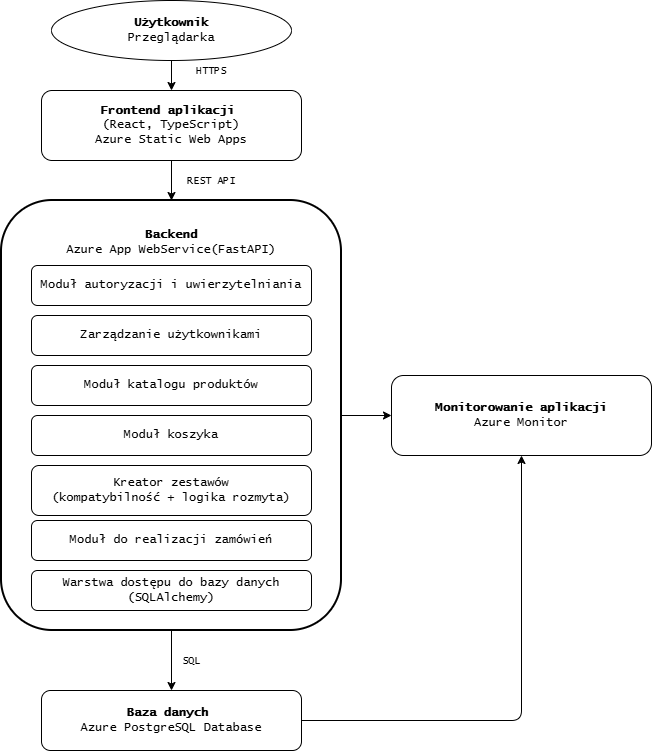
\includegraphics[width=\textwidth]{obrazki/diagram.png}
    \caption{Schemat działania aplikacji}
\end{figure}


% Diagram architektury (rysunek).
% Opis warstw: frontend, backend, baza danych.
% Komunikacja: REST API, JSON.
% Wdrożenie: Azure (baza, hosting).
\newpage
\subsection{Frontend}
Frontend aplikacji pełni ważną funkcję w funckjonowaniu każdego systemu, ponieważ odpowiada za prezentację danych dostarczonych z backendu. Projekt wykorzystuje nowoczesne technologie React, TypeScript oraz Vite, zapewniając innowacyjność, wydajność oraz skalowalność.
Inteligentny kreator zestawów komputerowych to jednostronicowy typ aplikacji webowej, dzięki czemu przełączanie widoku następuje dynamicznie bez konieczności ponownego ładowania zasobów. Takie rozwiązanie gwarantuje wysoką wydajność, prostotę oraz komfort użytkowania.
\\ Zadania realizowane przez interfejs:
\begin{itemize}
    \item prezentacja katalogu produktów, pobieranych dynamicznie z backendu,
    \item wybranie komponentów do przeniesienia z katalogu do kreatora,
    \item obsługa koszyka, dodawanie, modyfikowanie i usuwanie elementów,
    \item reakcja na działania użytkownika wykorzysując React Hooks,
    \item wyświetlanie aktualnego stanu kompatybilności zestawów,
    \item wykonywanie zapytań REST API do backendu w celu weryfikacji danych i aktualizacji stanu aplikacji.
\end{itemize}

Za wygląd zgodny ze standardami rynkowymi odpowiedzialny jest Tailwind CSS, gwarantując responwyność i estetykę rozwiązania. Framework umożliwia konfigurację i nadawanie stylów bezpośrednio w komponentach poprzez gotowe klasy utility. Takie rozwiązanie zapewnia intuicyjne i dynamiczne UI. Za komunikację z backendem odpowiada REST API poprzez zapytania realizowane biblioteką fetch API. Każda interakcja ze stroną powoduje wywołanie właściwego endpoint'u, co dynamicznie aktualizuje stan aplikacji, w tym bazę danych. Projekt wdrożony został w chmurze Microsoft Azure, jako Azure Static Web App, pełniącej rolę hostingu. Takie rozwiązanie umożliwia automatyzację CI/CD, co przekłada się na bezproblemowość i stabilność. Całość stacku techologicznego zapewnia wysoką dostępność aplikacji oraz łatwość korzystania i zarządzania.\\
Projekt frontendu powstał z myślą o:
\begin{itemize}
    \item przejrzystości interfejsu,
    \item prostocie korzystania,
    \item szybkości działania.
\end{itemize}  
Takie podejście powoduje, że aplikacja jest łatwa w utrzymaniu, skalowalna, wysoko dostępna oraz przejrzysta zarówno dla początkujących jak i zaawansowanych użytkowników.
% React + TypeScript, komponenty UI,
% kreator zestawów, interakcje z API.

\subsection{Backend}
% FastAPI – struktura endpointów
% Moduł produktu
% Moduł użytkownika
% Moduł kompatybilności
% Moduł koszyka / zamówień
Backend, jako jeden z filarów każdej aplikacji, odpowiada za logikę projektu, przetwarzanie danych oraz za kluczową komunikację kodu z bazą danych. Implementacja w języku Python, z wykorzystaniem frameworka FastAPI zapewnia nowoczesność i wydajność usług sieciowych, gwarantując przejrzystość, skalowalność oraz integralność z frontendem. Backend pełni funckję warstwy pośredniczącej pomiędzy interfejsem a bazą danych, gdzie żądania od strony użytkownika są nieustannie przetwarzane, a następnie przekazywane do odpowiednich modułów. Zwracana odpowiedź, w formacie JSON, umożliwia płynną komunikację w architekturze aplikacji.
\\
Struktura omawianej warstwy zawiera następujące moduły funckjonalne:
\begin{itemize}
    \item moduł autoryzacji i uwierzytelniania - odpowiada za rejestrację, logowanie i odpowiednie weryfikowanie danych użytkownika. Wykorzystuje algorytm bcrypt do zapewnienia bezpieczeństwa haseł,
    \item moduł zarządzania użytkownikami - umożliwia monitorowanie historii zamówień,
    \item moduł katalogu produktów - umożlliwia przeglądanie oferty sklepu, pobieranie listy części, filtrowanie i sortowanie,
    \item moduł kreatora - zapewnia możliwość zbierania danych o wybranych komponentach, gromadząc je w strukturze lokalnej sesji użytkownika, pozwalając na transport informacji z oferty do kreatora,
    \item moduł weryfikacji kompatybilności - odpowiada za porówywanie parametrów elementów zestawu, analizując zgodność pomiędzy nimi, stanowiąc rdzeń i główną funckjonalność projektu,
    \item moduł logiki rozmytej - odpowiedzialny jest za klasyfikację zestawu do jednej z kategorii,
    \item moduł koszyka i zamówień - zadaniem tego modułu jest dodawanie elementów do koszyka, nieustanne monitorowanie jego stanu i modyfikowanie zawartości.
\end{itemize}

Komunikacja pomiędzy backendem a bazą danych zaprojektowana została przy pomocy SQLAlchemy, który pełni funckję warstwy ORM. Takie rozwiązanie zapewnia odwzorowanie struktury tabel w postaci obiektów, znacząco ułatwiając implementację logiki, minimalizując ryzyko błędów oraz zwiększająć bezpieczeństwo. Operacje wykonywane w ten sposób określamy jako bezpieczne i atomowe. Wdrożenie w postaci Azure App Service, zapewnia skalowalność, prostotę utrzymania oraz wysoką dostępność, co jest niezwykle istotne podczas projektowania aplikacji przeznaczonej dla klientów. Uruchamianie nowych wersji odbywa się automatycznie poprzez mechanizm stałej implementacji i stałego dostarczania, znanego szerzej jako CI/CD.

\newpage

Backend zaprojektowany został z myślą o:
\begin{itemize}
    \item wysokiej wydajności,
    \item przejrzystości kodu,
    \item bezpieczeństwie danych,
    \item skalowalności,
    \item niezawodności,
    \item wysokiej dostępności.
\end{itemize}

Realiazcja tej części projektu w sposób opisany powyżej stanowi stabilną i skalowalną podstawę działania aplikacji, gwarantując poprawne komunikowanie się żądań użytkownika z bazą danych.
\subsection{Baza danych}
% PostgreSQL – organizacja danych
% Tabele i relacje w bazie
% Hosting w Microsoft Azure

Baza danych jest fundamentem każdej aplikacji biznesowej, gdyż odpowiedzialna jest za trwałe przechowywanie informacji o użytkownikach, produktach oraz zamówieniach. Zaprojektowana została  w oparciu o zasady normalizacji oraz analizę charakterystycznych właściwości komponentów, zapewniając integralność danych oraz efektywne weryfikowanie kompatybilności elementów.
\vspace{0.5cm}
\\
Model i schemat danych zaprojektowany został przy uzyciu Oracle SQL Developer Data Modeler, co umożliwiło utworzenie diagramu ERD oraz autmatyczne wygenerowanie definicji tabel. Wyeksportowana baza jako plik DDL wdrożona została do środowiska DataGrip, w którym wypełniono ją przygotowanymi INSERT'ami, zaciągniętymi z publicznego repozetorium komponentów\cite{pc_git}, w celu implementacji danych produktów. System operował w oparciu o PostgreSQL, pełniacy funkcję środowiska testowego wykorzystywanego do sprawnego implementowania backendu i modułów logiki. Gdy projekt przeszedł do etapu wdrożenia produkcyjnego, baza danych została zmigrowana do chmury Microsoft Azure, korzystając z gotowych poleceń podanych w dokumentacji Microsoft Azure\cite{azure_mig}. Przeniesiona struktura zaimplementowana została jako Azure PostgreSQL Database, co dzięki funkcjonalności grupowania zasobów Azure zapewnia integrację z produkcyjną wersją backendu uruchomioną w Azure App Service.
\newpage
Baza Danych spełnia wymagi trzeciej postaci normalnej (3NF), co oznacza, że nie zawiera redundancji danych, wszystkie atrybuty niekluczowe są w pełni zależne od klucza głównego właściwych tabel. Właściwość ta pozwala na:
\begin{itemize}
    \item zminimalizowanie ryzyka niespójnych danych,
    \item zwiększenie wydajności zapytań,
    \item eleminację duplikatów.
\end{itemize}
\vspace{0.5cm}

Kluczową rolę w bazie danych pełni tabela Produkty, bedąc ogólnym rejestrem wszystkich komponentów dostępnych w ofercie. Przechowuje ona podstawowe informacje o produktach, natomiast szczegółowe parametry znajdują się w dedykowanych tabelach zależnych od typu podzespołu. Takie rozwiązanie eleminuje redundację danych oraz dodaje przejrzystości do przechowywania właśiwości.
\vspace{0.5cm}
\\
W celu przechowywania wielu komponentów w jednym zestawie, koszyku lub zamówieniu zastosowano liczne relacje typu M:N, które zostały zrealizowane przy pomocy tabel łączących. Całość struktury została zabezpieczona kluczami obcymi, co zapewnia pełną integralność referencyjną oraz uniemożliwia tworzenie błędnych powiązań między danymi. Modularny charakter modelu umożliwia jego dalszy rozwój, w tym dodawanie nowych typów komponentów.
\vspace{0.5cm}
\\
Dzięki zastosowaniu odpowiednich narzędzi, normalizacji oraz chmurowej infrastruktury Azure, baza danych stanowi stabilny i skalowalny fundament systemu, wspierający zarówno logikę kompatybilności, jak i zarządzanie koszykami, zamówieniami oraz zestawami użytkowników.
\subsection{Infrastruktura chmurowa}
Wybór infranstruktury chmurowej jest podstawowym aspketem każdego nastawionego na wysoką dostepność projektu. Chmura Microsoft Azure gwarantuje skalowalność i bezpieczne środowisko, umożliwiając integrację z poszczególnymi komponentami systemu oraz automatyzację wdrażania kolejnych części aplikacji.

Organizację pracy znacząco upraszcza ulokowanie środowiska produkcyjnego w oparciu o grupę zasobów Azure, która zbiera całość w jednej strukturze administracyjnej. Takie rozwiązanie gwarantuje intuicyjne i kontrolowane zarządzanie usługami, co pozwala nieprzerwanie monitorować zużycie zasobów oraz koszty serwisu.
\newpage
Projekt operował na kredytach Azure o równowartości 100 USD, przyznanych przez Microsoft w ramach programu Azure for Students, pozwalając na wdrożenie aplikacji bez generowania dodatkowych kosztów. Środki te umożliwiły
uruchomienie wszystkich wymaganych usług, takich jak:
\begin{itemize}
    \item Azure App Service,
    \item Azure Static Web App,
    \item Azure Database for PostgreSQL.
\end{itemize}

\subsubsection{Azure Static Web App}
Warstwa frontend'u zaimplementowana została w usłudze Static Web Apps, co umożliwiło prezentowanie strony w sieci Internet. Usługa ta obsługuje:
\begin{itemize}
    \item automatyzację CI/CD,
    \item integrację z backendem.
\end{itemize}
\vspace{0.5cm}
Stanowi to lekkie, skalowalne rozwiązanie, zapewniając obsługę wielu użytkowników jednocześnie.
\subsubsection{Azure App Service}
Warstwa backend'u została wdrożona przy użyciu usługi App Service. Oparty na frameworku'u FastAPI i języku Python osadzona została jako aplikacja, działając na serwerze automatyzowanym przez usługi Azure, zapewniając dzięki temu:
\begin{itemize}
    \item uproszczone wdrażanie aktualizacji,
    \item zarządzanie środowiskiem wykonawczym,
    \item integrację z usługami monitorującymi Azure,
    \item stabilność,
    \item wysoką dostępność.
\end{itemize}
\vspace{0.5cm}
Takie rozwiązanie uodparnia backend na obciążenia i znacząco redukuje wkład użytkownika w administrację w czasie rzeczywistym.
\subsubsection{Azure Database for PostgreSQL}
Dane o podzespołach przetrzymywane są w usłudze Azure Database for PostgreSQL, zapewniając środowisko do zarządzania relacyjnymi bazami danych. Wdrożenie polegało na zmigrowaniu bazy PostgreSQL do Azure \cite{azure_mig}, obejmując elementy takie jak:
\begin{itemize}
    \item eskport struktury i danych,
    \item dostosowanie typów danych,
    \item weryfikację integralności.
\end{itemize}

Rozwiązanie to zapewnia dostęp do bazy z dowolnego urządzenia, gwarantując elastyczność pracy i wysoką niezawodność. Przetrzymywanie danych w chmurze daje możliwość elastycznego dostępu do danych zależnie od potrzeb, redukując koszty utrzymania. 

\subsubsection{Azure Monitor}
Aplikacja jest monitorowana w czasie rzeczywistym za pomocą usług:
\begin{itemize}
    \item Azure Monitor,
    \item Aplication Insights.
\end{itemize}
Takie rozwiązanie umożliwia nieustanne wykrywanie problemów, reagowanie na zwiększony ruch oraz automatyzację dopasowywania zasobów do aktualnych potrzeb.

\subsubsection{Koszty i optymalizacja}
W trakcie wdrażania przeanalizowany został potencjalny koszt utrzymania aplikacji, dobierając odpowiednie rozwiązania, o możliwie niskich paramterach z uwagi na niski poziom ruchu na stronie. Wprowadzone modyfikacje nie mają wpływu na funkcjonalność, pozwalają one na oszczędność środków, których zużycie nawet na średnich komponentach przekracza założony budżet. Wybrane do tego zostały następujące rozwiązania:
\begin{itemize}
    \item wybranie maszyny wirtualnej o najniższych możliwych parametrach,
    \item ustawienie automatycznego usypiania systemu w przypadku ruchu poniżej progu zdefiniowanego ręcznie,
    \item ograniczenie ruchu sieciowego do testowej podsieci wirutalnej.
\end{itemize}

W ten sposób możliwe stało się zmieszczenie w oferowanych przez Microsoft kredytach, ale również przygotowało projekt do ewentualnych przyszłych modyfikacji.
\subsubsection{Architektura logiczna}
Infrastruktura została umieszczona w jednej grupie zasobów, umożliwiając spójne zarządzanie, wzajemny dostęp do zasobów oraz przystępną modyfikacje pojedyńczych modułów.
Działanie infrastruktury przebiega w następujący sposób:
\begin{itemize}
    \item połączenie użytkownika z frontendem (Static Web App),
    \item komunikacja na linii frontend - backend (RestAPI),
    \item komunikacja na linii backend - Baza PostgreSQL,
    \item monitorowanie komponentów, zwracanie dedykowanych logów, które analizowane przez Azure Monitor dostosowywują parametry aplikacji.
\end{itemize}
Taki sposób implementacji zapewnia wysoką wydajność, stabilność, skalowalność oraz integralność, czyniąc aplikację gotową do działania w produkcyjnym środowisku.
\newpage
\section{Baza danych}
% Opis danych wykorzystywanych w systemie
% Główne encje: procesory, płyty główne, GPU, RAM, zasilacze...

\subsection{Model danych - ERD}

\begin{figure}[H]
    \centering
    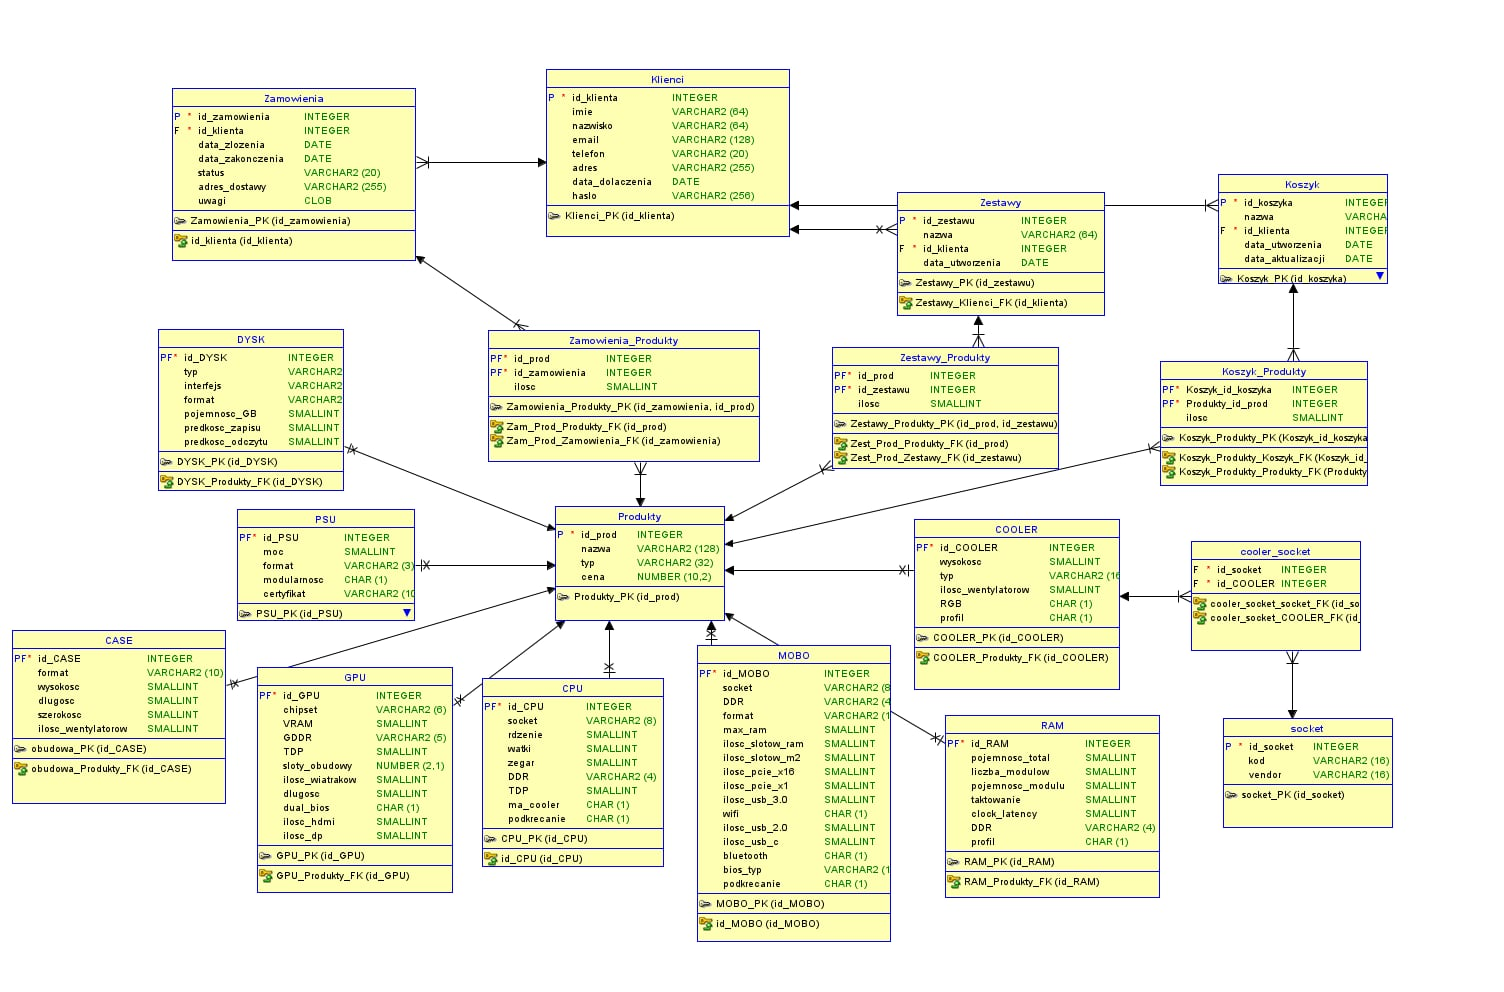
\includegraphics[width=\textwidth]{obrazki/erd.jpg} % tu ścieżka do Twojego pliku
    \caption{Diagram ERD bazy danych}
    \label{fig:erd}
\end{figure}

Na rysunku przedstawiono diagram ERD bazy danych systemu sklepu komputerowego 
z kreatorem zestawów PC. Model odzwierciedla główne obszary funkcjonalne:
aplikacji
\begin{itemize}
    \item zarządzanie klientami,
    \item zarządzanie produktami,
    \item zarządzanie koszykami,
    \item zarządzanie zamówieniami.
\end{itemize}

Centralne miejsce w diagramie zajmuje tabela Produkty, pełniąca rolę nadrzędnego 
rejestru wszystkich pozycji dostępnych w systemie. Zawiera ona podstawowe 
informacje o każdym produkcie, takie jak nazwa, typ oraz cena, natomiast 
szczegółowe parametry techniczne przechowywane są w dedykowanych tabelach 
odpowiadających konkretnym kategoriom sprzętu: CPU, GPU, RAM, MOBO, PSU, 
COOLER, DYSK oraz CASE. Każda z tych tabel posiada klucz obcy wskazujący na 
rekord w tabeli Produkty, co pozwala uniknąć redundancji danych oraz ułatwia 
zarządzanie wspólnymi atrybutami produktów.
\newpage 
Relacje związane z procesem zakupowym odwzorowane są poprzez tabele Klienci, 
Koszyk, Zamówienia oraz Zestawy. Każdy klient może posiadać wiele koszyków, 
zamówień oraz zapisanych zestawów, co odzwierciedlono relacjami 1:N. 
Zawartość koszyka, zamówienia oraz zestawu została zrealizowana za pomocą tabel 
łączących Koszyk\_Produkty, Zamówienia\_Produkty oraz Zestawy\_Produkty, które 
przechowują pary identyfikatorów produktu i obiektu nadrzędnego wraz z 
informacją o liczbie sztuk. Umożliwia to poprawne odwzorowanie relacji 
wiele-do-wielu pomiędzy produktami a koszykami, zamówieniami i zestawami.
\vspace{0.5cm}
\\
Istotnym elementem modelu są tabele socket oraz cooler\_socket, pełniące rolę 
słowników technicznych wykorzystywanych w logice kompatybilności. Tabela 
socket przechowuje informacje o typach gniazd procesorów, natomiast tabela 
cooler\_socket łączy coolery z obsługiwanymi przez nie socketami. Rozwiązanie to 
umożliwia powiązanie procesorów, płyt głównych oraz systemów chłodzenia oraz 
ułatwia implementację reguł sprawdzających zgodność komponentów.
\vspace{0.5cm}
\\
Zaprojektowany model danych zachowuje spójność referencyjną dzięki zastosowaniu 
kluczy głównych i obcych, a rozdzielenie danych ogólnych i szczegółowych na 
osobne tabele umożliwia utrzymanie bazy w co najmniej trzeciej postaci normalnej. 
Takie podejście ułatwia dalszą rozbudowę systemu o nowe typy podzespołów oraz 
dodatkowe funkcje biznesowe, jednocześnie zapewniając integralność i wysoką 
jakość przechowywanych danych.


\newpage 

\subsection{Opis najważniejszych encji}

\subsubsection{Tabela produkty}

Najbardziej istotną, pełniącą funkcję głównej, tabelą w całej bazie danych jest tabela produkty. Kluczem tabeli jest id\_prod, klucz ten podstawą działania aplikacji. Encja produkty zawiera również pełną nazwę produktu w typie varchar, typ produktu, który umożliwia prowadzenie poprawnych operacji w kreatorze zestawów, stanowiąc pole odpowiedzialne za łączenie odpowiednich tabel z dodatkowymi danymi konkrentego produktu, zależnie od jego rodzaju. Tabela zawiera również kolumnę cena w typie numeric, który wybrano w celu zachowania spójności działania programu.
\begin{figure}[H]
    \centering
    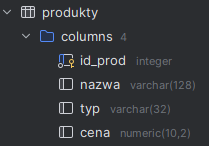
\includegraphics[width=\textwidth]{obrazki/tabela_produkty.png} % tu ścieżka do Twojego pliku
    \caption{Tabela Produkty w programie DataGrip}
    \label{fig:tabela_produkty}
\end{figure}

\newpage 

\subsubsection{Tabela Klienci}
\begin{figure}[H]
    \centering
    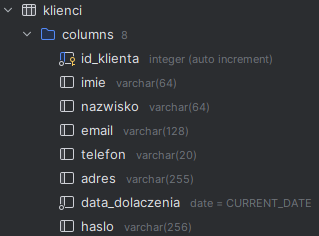
\includegraphics[width=\textwidth]{obrazki/tabela_klienci.png} % tu ścieżka do Twojego pliku
    \caption{Tabela Klienci w programie DataGrip}
    \label{fig:tabela_klienci}
\end{figure}

\newpage 
\subsubsection{Tabela Koszyk}
\begin{figure}[H]
    \centering
    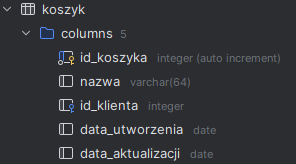
\includegraphics[width=\textwidth]{obrazki/tabela_koszyk.png} % tu ścieżka do Twojego pliku
    \caption{Tabela Koszyk w programie DataGrip}
    \label{fig:tabela_koszyk}
\end{figure}

\newpage 
\subsubsection{Tabela Zamówienia}
\begin{figure}[H]
    \centering
    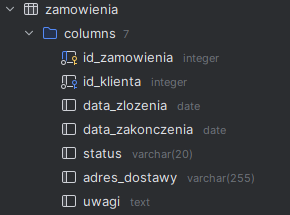
\includegraphics[width=\textwidth]{obrazki/tabela_zamowienia.png} % tu ścieżka do Twojego pliku
    \caption{Tabela Zamówienia w programie DataGrip}
    \label{fig:tabela_zamowienia}
\end{figure}

\newpage 
\subsubsection{Tabela Zestawy}
\begin{figure}[H]
    \centering
    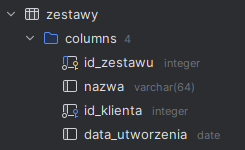
\includegraphics[width=\textwidth]{obrazki/tabela_zestawy.png} % tu ścieżka do Twojego pliku
    \caption{Tabela Zestawy w programie DataGrip}
    \label{fig:tabela_zestawy}
\end{figure}
\newpage 
\subsubsection{Tabela GPU}
\begin{figure}[H]
    \centering
    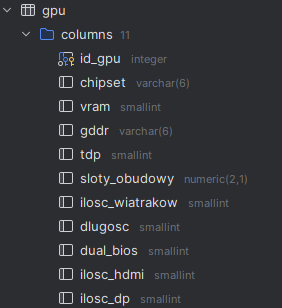
\includegraphics[width=\textwidth]{obrazki/tabela_gpu.png} % tu ścieżka do Twojego pliku
    \caption{Tabela GPU w programie DataGrip}
    \label{fig:tabela_gpu}
\end{figure}

\newpage 
\subsubsection{Tabela CPU}
\begin{figure}[H]
    \centering
    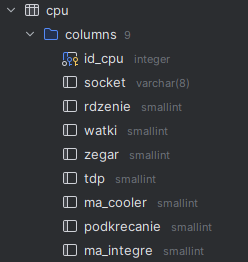
\includegraphics[width=\textwidth]{obrazki/tabela_cpu.png} % tu ścieżka do Twojego pliku
    \caption{Tabela CPU w programie DataGrip}
    \label{fig:tabela_cpu}
\end{figure}

\newpage 
\subsubsection{Tabela MOBO}
\newpage 
\begin{figure}[H]
    \centering
    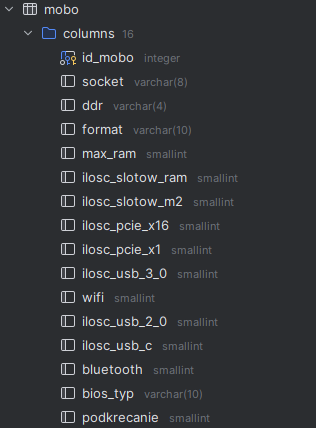
\includegraphics[width=\textwidth]{obrazki/tabela_mobo.png} % tu ścieżka do Twojego pliku
    \caption{Tabela MOBO w programie DataGrip}
    \label{fig:tabela_mobo}
\end{figure}

\newpage 
\subsubsection{Tabela RAM}
\begin{figure}[H]
    \centering
    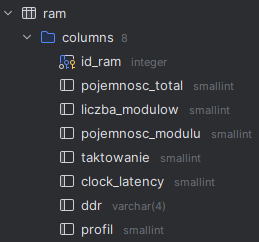
\includegraphics[width=\textwidth]{obrazki/tabela_ram.png} % tu ścieżka do Twojego pliku
    \caption{Tabela RAM w programie DataGrip}
    \label{fig:tabela_ram}
\end{figure}

\newpage 
\subsubsection{Tabela PSU}
\begin{figure}[H]
    \centering
    
\includegraphics[width=\textwidth]{obrazki/tabela_psu.png} % tu ścieżka do Twojego pliku
    \caption{Tabela PSU w programie DataGrip}
    \label{fig:tabela_psu}
\end{figure}

\newpage 
\subsubsection{Tabela Cooler}
\begin{figure}[H]
    \centering
    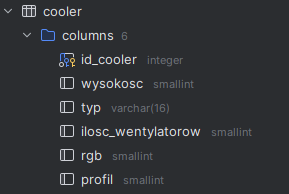
\includegraphics[width=\textwidth]{obrazki/tabela_cooler.png} % tu ścieżka do Twojego pliku
    \caption{Tabela Cooler w programie DataGrip}
    \label{fig:tabela_cooler}
\end{figure}

\newpage 
\subsubsection{Tabela Dysk}
\begin{figure}[H]
    \centering
    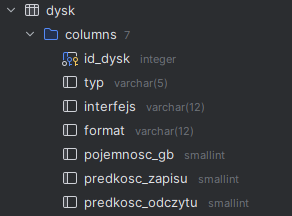
\includegraphics[width=\textwidth]{obrazki/tabela_dysk.png} % tu ścieżka do Twojego pliku
    \caption{Tabela Dysk w programie DataGrip}
    \label{fig:tabela_dysk}
\end{figure}


% Każda encja w 2–3 zdaniach:
% Produkty, Kategorie, Użytkownicy, Zamówienia, Parametry techniczne.

\section{Komponenty i moduły systemu}

\subsection{Moduł kompatybilności podzespołów}
% Jak sprawdzana jest zgodność: socket, DDR, TDP, format, VRM, chłodzenie.
% Kolejność weryfikacji.

\subsection{Moduł logiki rozmytej}
% Opis funkcji przynależności,
% Kategorie: budżetowy / wydajny / energooszczędny,
% Zastosowanie logiki rozmytej do klasyfikacji zestawu.

\subsection{Moduł zarządzania koszykiem i zamówieniami}
% Dodawanie, modyfikacja, finalizacja,
% przepływ danych.

\section{Najważniejsze algorytmy}
% Algorytm sprawdzania kompatybilności (pseudokod / schemat blokowy)
% Algorytm klasyfikacji logiką rozmytą

\section{Diagramy UML}
% Use Case (opcjonalnie – masz już w R3)
% Sequence diagram (np. „budowa zestawu i weryfikacja”)
% Class diagram (opcjonalnie)

\section{Szczegóły implementacji wybranych elementów}
% Kod / fragmenty implementacji (krótko)
% Architektura folderów backendu i frontendu
% Wzorce projektowe (jeśli używasz np. repository pattern)

\newpage


% TODO
\chapter{Weryfikacja i walidacja}
\label{ch:06}
% \begin{itemize}
% \item sposób testowania w ramach pracy (np. odniesienie do modelu V)
% \item organizacja eksperymentów
% \item przypadki testowe zakres testowania (pełny/niepełny)
% \item wykryte i usunięte błędy
% \item opcjonalnie wyniki badań eksperymentalnych
% \end{itemize}

\section{Cel weryfikacji systemu}
% Krótki opis po co testujemy, jakie aspekty miały być zweryfikowane:
% - poprawność działania,
% - kompletność funkcjonalności,
% - zgodność z wymaganiami,
% - poprawność logiki kompatybilności,
% - stabilność backendu i frontendu.

\section{Metody testowania}
% Jak testowałeś system:
% - testy funkcjonalne,
% - testy integracyjne (backend + baza),
% - testy API (np. Postman),
% - testy walidacyjne dotyczące kompatybilności,
% - testy manualne frontendu.
% Opcjonalnie model V lub diagram procesu testowania.

\section{Organizacja eksperymentów}
% Co konkretnie było sprawdzane:
% - logowanie / rejestracja,
% - pobieranie danych o produktach,
% - dodawanie komponentów do zestawu,
% - działanie algorytmu kompatybilności,
% - działanie logiki rozmytej,
% - realizacja zamówienia.
% Jak wyglądało środowisko testowe:
% - Azure (baza),
% - lokalny backend / production build frontendu.

\section{Przypadki testowe}
% W tej sekcji opisujesz tabelki testów.
% Minimum 6–10 przypadków.
% Np.:
% - Zestaw kompatybilny → wynik pozytywny,
% - CPU AM5 + Mobo LGA1700 → wynik negatywny,
% - RAM DDR5 + Mobo DDR4 → negatywny,
% - GPU za długie do obudowy → negatywny,
% - Zbyt słaby PSU do CPU/GPU → negatywny,
% - Poprawna rejestracja,
% - Błędne logowanie.
% Można przedstawić jako tabela w LaTeX.

\section{Wyniki testów}
% Tutaj opisujesz:
% - ile testów przeszło pozytywnie,
% - jakie błędy wykryto podczas testów,
% - które elementy wymagały poprawy,
% - np. błędne zapytanie SQL, błąd walidacji, źle przekazywany parametr.

\begin{table}[H]
\centering
\caption{Przykładowe wyniki testów kompatybilności zestawów komputerowych.}
\label{tab:kompatybilnosc}
\begin{tabular}{|p{0.8cm}|p{2.6cm}|p{3.6cm}|p{3.2cm}|p{2.8cm}|}
\hline
\textbf{ID} & \textbf{Test} & \textbf{Dane wejściowe} & \textbf{Problem} & \textbf{Wynik} \\
\hline
1  & CPU + płyta główna & Ryzen 5 7600 + B650 & Brak & Kompatybilne \\
\hline
2  & CPU + płyta główna & i5-12600K + B550 & Różne sockety & Niekompatybilne \\
\hline
3  & RAM + płyta główna & DDR5 6000 + B460 & RAM DDR5 + MOBO DDR4 & Niekompatybilne \\
\hline
4  & GPU + obudowa & RTX 4070 (330 mm) + obudowa 300 mm & Zbyt długie GPU & Niekompatybilne \\
\hline
5  & Zasilacz + CPU/GPU & PSU 400W + RTX 3080 & Zbyt mała moc & Niekompatybilne \\
\hline
6  & Chłodzenie + socket & Cooler AM4 + CPU LGA1700 & Niezgodne typy chłodzenia & Niekompatybilne \\
\hline
7  & Zestaw kompletny & CPU + GPU + RAM + Mobo + PSU zgodne & Brak & Kompatybilne \\
\hline
8  & Zestaw błędny & 3 niezgodności (DDR, TDP, GPU) & Złożona & Niekompatybilne \\
\hline
\end{tabular}
\end{table}

\section{Wykryte i usunięte błędy}
% Wypisz realne rzeczy, które musiałeś naprawić w kodzie:
% - błędne mapowanie z SQLAlchemy,
% - literówki w endpointach,
% - błędy konfiguracji .env,
% - problemy z CORS,
% - dane testowe, które łamały algorytm kompatybilności.
% To zawsze robi super wrażenie na promotorze.

\section{Ocena poprawności działania systemu}
% Podsumowanie tego, co udało się potwierdzić:
% - system prawidłowo weryfikuje kompatybilność,
% - frontend poprawnie prezentuje wyniki,
% - API działa stabilnie,
% - dane w bazie zgodne ze strukturą ERD.
% Wskazujesz tu, że cele pracy zostały potwierdzone.


\chapter{Podsumowanie i wnioski}

% TODO

% \begin{itemize}
% \item uzyskane wyniki w świetle postawionych celów i zdefiniowanych wyżej wymagań
% \item kierunki ewentualnych danych prac (rozbudowa funkcjonalna …)
% \item problemy napotkane w trakcie pracy
% \end{itemize}

Celem niniejszego rozdziału jest podsumowanie rezultatów uzyskanych podczas realizacji projektu oraz ocena stopnia spełnienia celów pracy. Dodatkowo przedstawiono wnioski dotyczące dalszego możliwego rozwoju systemu oraz trudności napotkane w trakcie implementacji.

\section{Realizacja celów pracy}
% Tutaj wpisz 1–2 akapity o tym:
% - które cele zostały spełnione (np. baza, backend, weryfikacja kompatybilności, logika rozmyta, frontend)
% - co działa zgodnie z założeniami
% - jak system odpowiada na problem przedstawiony w rozdziale 1

\section{Ocena otrzymanych rezultatów}
% Tutaj wpisz:
% - ogólną ocenę jakości systemu
% - jak system sprawdza się w praktyce
% - jakie funkcje działają najlepiej
% - jakie są mocne strony rozwiązania (kompatybilność, API, UX, Azure)

\section{Trudności napotkane podczas realizacji}
% Wypisz, co było trudne:
% - integracja backendu z bazą
% - różne typy danych w parametrach sprzętu
% - projekt logiki kompatybilności
% - wdrożenie Azure / problemy z konfiguracją
% - frontend + backend komunikacja, CORS itp.

\section{Możliwe kierunki dalszego rozwoju}
% Tutaj wpisujesz, co można dodać w przyszłości:
% - rozbudowa logiki rozmytej (więcej kategorii, bardziej precyzyjne reguły)
% - automatyczne dobieranie podzespołów pod budżet
% - integracja z zewnętrznymi API sklepów
% - rekomendacje AI / ML
% - wersja mobilna aplikacji
% - panel administratora i zarządzanie katalogiem
% - testy automatyczne i CI/CD

\section{Wnioski końcowe}
% 1–2 akapity:
% - ogólne podsumowanie
% - co projekt wnosi
% - potwierdzenie znaczenia rozwiązania
% - że system spełnia założenia i jest praktycznie użyteczny

\backmatter
	
\cleardoublepage
\phantomsection
%\bibliographystyle{plplain}  % bibtex
%\bibliography{biblio} % bibtex
\addcontentsline{toc}{chapter}{Bibliografia}
\printbibliography           % biblatex
	
\begin{appendices}

% TODO
\chapter{Spis skrótów i symboli}

\begin{itemize}

\item[API] interfejs programistyczny aplikacji (ang. \english{Application Programming Interface})
\item[ASGI] asynchroniczny interfejs serwera aplikacji (ang. \english{Asynchronous Server Gateway Interface})
\item[ATX] standard rozmiaru płyt głównych i obudów komputerowych (ang. \english{Advanced Technology eXtended})
\item[CPU] procesor centralny (ang. \english{Central Processing Unit})
\item[CRUD] podstawowe operacje na danych: tworzenie, odczyt, modyfikacja, usuwanie (ang. \english{Create, Read, Update, Delete})
\item[CSS] kaskadowe arkusze stylów (ang. \english{Cascading Style Sheets})
\item[DDR] standard pamięci RAM \english{(Double Data Rate)}
\item[ERD] diagram związków encji (ang. \english{Entity–Relationship Diagram})
\item[GPU] procesor graficzny (ang. \english{Graphics Processing Unit})
\item[HTML] język znaczników stron WWW (ang. \english{HyperText Markup Language})
\item[HTTP] protokół komunikacji klient-serwer (ang. \english{HyperText Transfer Protocol})
\item[JSON] format danych tekstowych (ang. \english{JavaScript Object Notation})
\item[ORM] mapowanie obiektowo-relacyjne (ang. \english{Object–Relational Mapping})
\item[PSU] zasilacz komputerowy (ang. \english{Power Supply Unit})
\item[RAM] pamięć operacyjna (ang. \english{Random Access Memory})
\item[REST] styl architektury usług sieciowych (ang. \english{Representational State Transfer})
\item[SQL] język zapytań do baz danych (ang. \english{Structured Query Language})
\item[SSD] dysk półprzewodnikowy (ang. \english{Solid State Drive})
\item[TDP] maksymalna ilość ciepła odprowadzana przez układ (ang. \english{Thermal Design Power})
\item[TS] język programowania TypeScript (ang. \english{TypeScript})
\item[UI] interfejs użytkownika (ang. \english{User Interface})
\item[UML] zunifikowany język modelowania (ang. \english{Unified Modeling Language})
\item[URL] adres zasobu internetowego (ang. \english{Uniform Resource Locator})
\item[WWW] ogólnoświatowa sieć internetowa (ang. \english{World Wide Web})

\end{itemize}



% TODO
\chapter{Źródła}

Jeżeli w pracy konieczne jest umieszczenie długich fragmentów kodu źródłowego, należy je przenieść w to miejsce.

\begin{lstlisting}
if (_nClusters < 1)
	throw std::string ("unknown number of clusters");
if (_nIterations < 1 and _epsilon < 0)
	throw std::string ("You should set a maximal number of iteration or minimal difference -- epsilon.");
if (_nIterations > 0 and _epsilon > 0)
	throw std::string ("Both number of iterations and minimal epsilon set -- you should set either number of iterations or minimal epsilon.");
\end{lstlisting}


% % % % % % % % % % % % % % % % % % % % % % % % % % % % % % % % % % % 
% Pakiet minted wymaga odkomentowania w pliku config/settings.tex   %
% importu pakietu minted: \usepackage{minted}                       %
% i specjalnego kompilowania:                                       %
% pdflatex -shell-escape praca                                      %
% % % % % % % % % % % % % % % % % % % % % % % % % % % % % % % % % % % 

%\begin{minted}[linenos,breaklines,frame=lines]{c++}
%if (_nClusters < 1)
%   throw std::string ("unknown number of clusters");
%if (_nIterations < 1 and _epsilon < 0)
%   throw std::string ("You should set a maximal number of iteration or minimal difference -- epsilon.");
%if (_nIterations > 0 and _epsilon > 0)
%   throw std::string ("Both number of iterations and minimal epsilon set -- you should set either number of iterations or minimal epsilon.");
%\end{minted}


% TODO
\chapter{Lista dodatkowych plików, uzupełniających tekst pracy} 


W systemie do pracy dołączono dodatkowe pliki zawierające:
\begin{itemize}
\item źródła programu,
\item dane testowe,
\item film pokazujący działanie opracowanego oprogramowania lub zaprojektowanego i~wykonanego urządzenia,
\item itp.
\end{itemize}


\listoffigures
\addcontentsline{toc}{chapter}{Spis rysunków}
\listoftables
\addcontentsline{toc}{chapter}{Spis tabel}

\end{appendices}

\end{document}


%% Finis coronat opus.

